%1521001##1##.tex
\documentclass[12pt,letterpaper]{article}
\usepackage{mathptmx}
\usepackage[margin=1in]{geometry}

\usepackage{setspace}
\singlespacing
  
\usepackage{amssymb,latexsym}
\usepackage[round,sort]{natbib}
\usepackage{fancyhdr}
\usepackage{lastpage}
\usepackage{graphicx,multirow}
\graphicspath{ {qe1/} }

% Bold Table and Figure captions
\usepackage{caption}
\captionsetup{figurename=FIGURE}
\captionsetup{tablename=TABLE}
\captionsetup[figure]{labelfont=bf}
\captionsetup[table]{labelfont=bf}
  
% Turns off all section numbering
\setcounter{secnumdepth}{0} 

  % Places all tables at end of document and creates AOM-style table-here placeholders
  \usepackage[nolists]{endfloat} % Places all figures and charts at end of manuscript and adds 'insert table x about here' lines.
  \renewcommand{\figureplace}{
    \begin{center}
    \begin{singlespace}
    ------------------------------------\\
    Insert \figurename \ \thepostfig\ about here.\\
    ------------------------------------
    \end{singlespace}
    \end{center}}
  \renewcommand{\tableplace}{%
    \begin{center}
    \begin{singlespace}
    ------------------------------------\\
    Insert \tablename \ \theposttbl\ about here.\\
    ------------------------------------
    \end{singlespace}
    \end{center}}

  \usepackage{titlesec}
   \titleformat{\title}
       {\filcenter\normalfont\bfseries\uppercase}{\thetitle}{1em}{}
  \titleformat{\section}
    {\filcenter\normalfont\bfseries\uppercase}{\thesection}{1em}{}
  \titleformat{\subsection}
    {\normalfont\bfseries}{\thesubsection}{1em}{}
  \titleformat{\subsubsection}[runin]
   {\normalfont\bfseries\slshape}{\thesubsubsection}{1em}{\hspace*{\parindent}}
       
\usepackage{tabu}
\usepackage{textcomp}
\usepackage{listings}
\usepackage{hyperref}
\usepackage{verbatim}
\usepackage{tabu}
\hypersetup{
    colorlinks=true,
    linkcolor=blue,
    filecolor=cyan,      
    urlcolor=cyan,
    citecolor=blue,
}

\usepackage{etoolbox}

\makeatletter

% Patch case where name and year are separated by aysep
\patchcmd{\NAT@citex}
  {\@citea\NAT@hyper@{%
     \NAT@nmfmt{\NAT@nm}%
     \hyper@natlinkbreak{\NAT@aysep\NAT@spacechar}{\@citeb\@extra@b@citeb}%
     \NAT@date}}
  {\@citea\NAT@nmfmt{\NAT@nm}%
   \NAT@aysep\NAT@spacechar\NAT@hyper@{\NAT@date}}{}{}

% Patch case where name and year are separated by opening bracket
\patchcmd{\NAT@citex}
  {\@citea\NAT@hyper@{%
     \NAT@nmfmt{\NAT@nm}%
     \hyper@natlinkbreak{\NAT@spacechar\NAT@@open\if*#1*\else#1\NAT@spacechar\fi}%
       {\@citeb\@extra@b@citeb}%
     \NAT@date}}
  {\@citea\NAT@nmfmt{\NAT@nm}%
   \NAT@spacechar\NAT@@open\if*#1*\else#1\NAT@spacechar\fi\NAT@hyper@{\NAT@date}}
  {}{}

\lstset{
basicstyle=\ttfamily,
columns=flexible,
breaklines=true
}
\newenvironment{hypothesis}{
  	\itshape
  	\leftskip=\parindent \rightskip=\parindent
  	\noindent\ignorespaces}

\fancypagestyle{plain}{
  \renewcommand{\headrulewidth}{0pt}
  \fancyhf{}
}	


\begin{document}
\title{Inducing Strategic Initiatives at a Startup Firm:\\Understanding the Role of the Co-founding Team}
\date{}
\maketitle

\begin{abstract} 
\normalsize 

\end{abstract}


{\textbf{Keywords:} \\\indent }

\newpage
\pagestyle{fancy}
\fancyhf{}
\lhead{Inducing Strategic Initiatives at a Startup Firm}
\rhead{\thepage}

\begin{center}
\textbf{Inducing Strategic Initiatives at a Startup Firm:\\Understanding the Role of the Co-founding Team}
\end{center}

In the form of a detailed literature review, describe the \cite{Lovas2000} model and compare it to prior models of \cite{Burgelman?} and \cite{Bower?}. Highlight the key aspects of the framework, how it is different and what salient aspects stand out that you then build on top of in this article. Suggest why you think \cite{Lovas2000} model is appropriate. Draw out a table Table ~\ref{payoffmatrix} that compares the various theories and their assumptions, traditions, and recommendations.

\begin{table}
\begin{centering}
\caption {Comparison}
\label{payoffmatrix}
{\tabulinesep=1.4mm
\begin{tabu}{|c|c|c|c|}
\hline
          & Bower Model & Burgelman Model & Lovas and Ghoshal Model \\
\hline   
    Tradition & Theta & Beta  & God \\
\hline    
    Assumptions & Alpha & Hexa  & None \\
\hline    
    Recommendations & Rationalist & Behavioral & Prgamatist \\
\hline 
\end{tabu}}

\end{centering}
\end{table} 

\section{Theory}
You also need to bring in literature discussing the phenomenon (startup firm strategy). Maybe look up strategy entrepreneurship journal.

\subsection{The \cite{Lovas2000} Model}
either redraw or paste the picture
\subsection{Variation, Selection, Retention}
Bring in the model here.

This should lead to the research question in the form of a gap in the current literature. Describe the question, and why it is important to study it (what additional insight will it provide, what policy/strategic implications will it have).

Develop hypotheses. Use theoretical arguments to lay out an interesting conundrum and then attempt to answer that in the form of propositions.
\subsection{On the topic of the general hypotheses}
 Figure ~\ref{fig:3a} lays out the average score charts for four agent-field combinations while enforcing the field to start in Right of Center (this is the same as saying $p_{0,F}^0 = 0.75$). 
\subsubsection{Leading into H1a}
We do so since the scale is symmetric across the Center (C), any initial mapping 

\begin{hypothesis}
{Hypothesis 1a: When the institutional field is open to influence, slow learning adversarial agents will raise overall performance higher than slow learning agents with a neutral orientation\\}
\end{hypothesis}

\subsubsection{Leading into H2a}
This trend is confirmed further in Figure ~\ref{fig:3a} where the learning rates of agents are increased even further to \textquotesingle Fast\textquotesingle .

\begin{hypothesis}
{Hypothesis 2a: For the same initial outcome preferences,  the overall performance score varies curvilinearly with difference in the rates of learning of the agent and the institutional field\\}
\end{hypothesis}

\section{Method}
Then describe an empirical setting in the form of a quasi-experimental setup where this will be examined.
\section{Sample Selection}
Use ideas from \cite{Burgelman1991} Implications

\section{Limitations and Future Work}
Suggest how this study may help inform the literatures that it is drawing from, and the interesting research avenues it will open up. Discuss level of generalizability.

\section{Notes}
\subsection{\cite{Lovas2000} Model}
The model consists five main elements, viz., (1) strategic initiatives and human and social capital, which are the units of selection; (2) strategic intent, which defines the objective function; (3) administrative systems, which facilitate the evolutionary process; sources of variation; and (5) agents of selection and retention in the evolutionary process, both which potentially include every employee of company.

\begin{figure}[h]
\begin{centering}
  \caption{The five elements of guided evolution, adopted from \cite{Lovas2000}}
  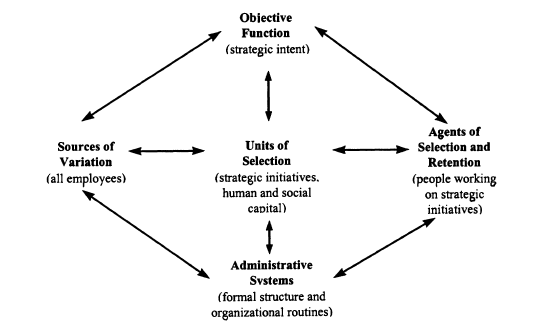
\includegraphics[width=\textwidth]{Lovas2000}
  \label{fig:Lovas2000}
\end{centering}
\end{figure}

\subsection{\cite{Burgelman1991} Propositions}
PROPOSITION 1. Firms that are relatively successful over long periods of time, say ten years or more, will be characterized by top managements that are concerned with building the quality of the organization's induced and autonomous strategic processes as well as with the content of the strategy itself.

\begin{figure}[h]
\begin{centering}
  \caption{Intraorganizational Ecology of Strategy Making and Organizational Adaptation, adopted from \cite{Burgelman1991}}
  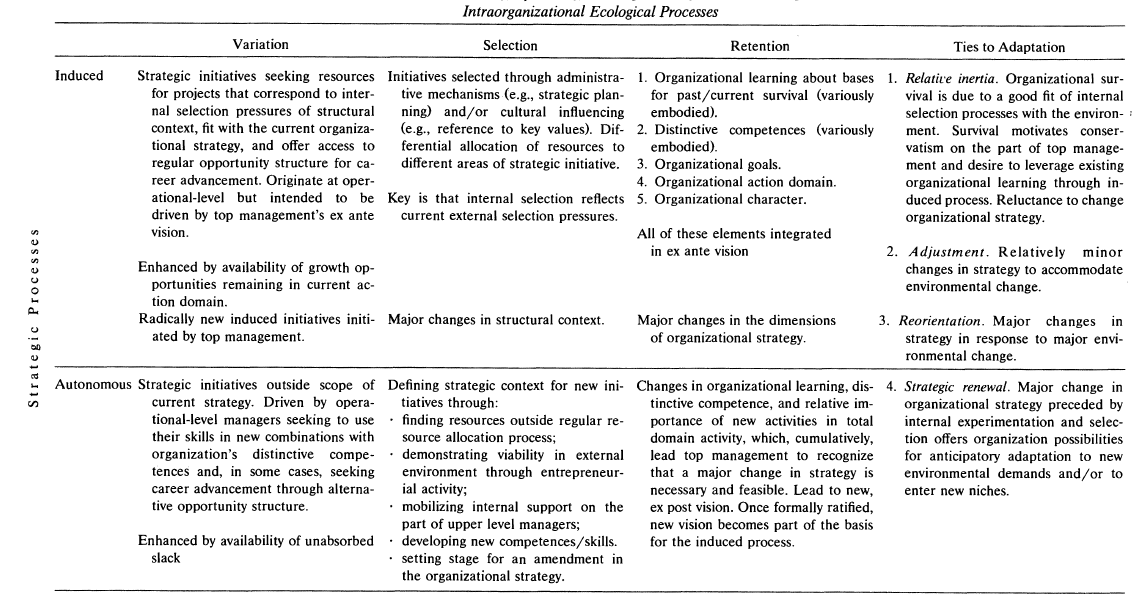
\includegraphics[width=\textwidth]{Burgelman1991}
  \label{fig:Burgelman1991}
\end{centering}
\end{figure}

PROPOSITION 2. Firms that are relatively successful over long periods of time, say ten years or more, will be characterized by maintaining top driven strategic intent while simultaneously maintaining bottoms-up driven internal experimentation and selection processes.

PROPOSITION 3. The population of firms with successful strategic reorientations will contain a significantly higher proportion of firms whose strategic reorientations were preceded by internal experimentation and selection processes than the population of firms with failing strategic reorientations.

\subsection{\cite{Burgelman1991} Conclusions}
The intraorganizational perspective on strategy making also extends frameworks presented by Mintzberg (1978) and Quinn (1982) in the strategic management literature. It does so by documenting more explicitly some of the sources of emergent strategy, by further elucidating the organizational decision processes through which emergent strategies become part of realized strategies (strategic context determination), by identifying feedback mechanisms between realized and intended strategy, and by providing some evidence that logical incrementalism is likely to be variation reducing and may need to be augmented with an autonomous strategic process to enhance long-term organizational survival. The perspective presented in the paper adds some additional dynamism to these earlier frameworks and draws more explicit attention to the simultaneity of multiple strategy-making processes in organizations.

\subsection{\cite{Burgelman1991} Implications}
future research could examine whether consistently successful firms are characterized by top managements' spending efforts on building each organization's strategy-making processes; whether such firms simultaneously exercise induced and autonomous strategic processes; and whether successful reorientations are more likely to be preceded by internal experimentation and selection processes effected through the autonomous strategic process than are the unsuccessful ones. Future research could also examine the possibilities that there may be an optimal level of ambiguity in the concept of strategy (March 1978) and an optimal degree of coupling in the structural context (Weick 1976). This would require studying the working of strategy-making processes in different types of organizations, such as generalists versus specialists (Freeman and Hannan 1983) or defenders, prospectors, analyzers and reactors (Miles and Snow 1978), and under different types of environmental conditions (e.g., Freeman and Hannan 1983, Eisenhardt 1989). 

\subsection{\cite{Burgelman1994} Model}
\begin{figure}[h]
\begin{centering}
  \caption{Forces driving the strategic business-exit process, adopted from \cite{Burgelman1994}}
  \includegraphics[width=\textwidth]{Burgelman1994}
  \label{fig:Burgelman1994}
\end{centering}
\end{figure}

\subsection{\cite{Mintzberg1978} Model}
Figure ~\ref{fig:Mintzberg1978} in the appendix displays the original resource allocation process suggested by \cite{Mintzberg1978}

\subsection{\cite{Quinn1980} Model}
Figure ~\ref{fig:Quinn1980a} and Figure ~\ref{fig:Quinn1980b} in the appendix displays the original resource allocation process suggested by \cite{Quinn1980}

\subsection{\cite{Bower1970} Model}
Figure ~\ref{fig:Bower1970} in the appendix displays the original resource allocation process suggested by \cite{Bower1970}

\subsection{\cite{Burgelman1983b} Model}
Figure ~\ref{fig:Burgelman1983b} in the appendix displays the Bower-Burgelman (B-B) model proposed by \cite{Burgelman1983b}

\subsection{\cite{Noda1996} Notes}
An explicit recognition of inherent organizational complexities, often described as 'possible goal incongruence,' 'information asymmetry,' and 'organizational politics' (e.g., Barnard, 1938; Simon, 1945; Cyert and March, 1963; Crozier, 1964), as well as 'unpredictable' and 'uncontrol- lable' environments (e.g., Schumpeter, 1934; Nelson and Winter, 1982; Thompson, 1967; Pfeffer and Salancik, 1978; Miles, 1982), has led some strategic management scholars to describe how strategy is actually formed instead of prescribing what it should be. Findings from their empirical studies suggest that strategy is, more or less, emergent from lower levels of organizations (e.g., Mintzberg, 1978; Pascale, 1984; Mintzberg and Waters, 1985), whether through trial-and-error learning (Mintzberg and McHugh, 1985), incrementally with logical guidance from the top (Quinn, 1980), or such that small changes are often punctuated by a sudden big change in a relatively short period (Miller and Friesen, 1984; Tushman and Romanelli, 1985; Gersick, 1991). From this strategy process perspective, strategy is 'a pattern in a stream of decisions and actions' (Mintzberg and McHugh, 1985: 161) that are distributed across multiple levels of an organization.

Whereas some of the scholars associated with this line of research see the process as unguided or 'muddling through' (e.g., Lindbloom, 1959; Wrapp, 1967), others see part of top manage- ment's task as intervening in the emergent strat- egy process and attempting to maneuver the enterprise to a preferable course of direction. These scholars explore multilevel managerial activities that shape the strategy process, inter- acting with external and internal forces. Bower (1970) initiated this line of inquiry by conducting an intensive field-based study on strategic planning and capital investment in a large, diversified firm and presenting a parsimonious framework, grounded in the field data, for understanding the interplay of those managerial activities. His pro- cess model was validated by subsequent field studies in different organizational settings and on various strategic processes (see Bower and Doz, 1979, for the details of these studies). It was then further extended by Burgelman (1983a) in his clinical study on internal corporate venturing (ICV) in a large corporation.

The Bower-Burgelman (B-B) process model of strategy making in a large, complex firm depicts multiple, simultaneous, interlocking, and sequential managerial activities over three levels of organizational hierarchy (i.e., front-line or bot- tom, middle, and top managers) and concep- tualizes intraorganizational strategy-making pro- cesses as consisting of four subprocesses: two interlocking bottom-up core processes of 'defi- nition' and 'impetus' and two overlaying corpor- ate processes of 'structural context determination' and 'strategic context determination.' Definition is a cognitive process in which technological and market forces, initially ill defined, are communi- cated to the organization, and strategic initiatives are developed primarily by front-line managers who usually have specific knowledge on tech- nology and are closer to the market (Chakravarthy and Lorange, 1991; Jensen and Meckling, 1992). Impetus is a largely sociopolitical process by which these strategic initiatives are continually championed by front-line managers, and are adopted and brokered by middle managers who, in doing so, put their reputations for good judg- ment and organizational career at stake. The role of top managers is limited in that they do not necessarily have the appropriate knowledge or information to evaluate technical and economic aspects of the strategic initiatives, and tend to rely on the track records or credibility of propos- ing middle managers in making resource allo- cation decisions (Bower, 1970).

Strategic initiatives therefore 'emerge' pri- marily from managerial activities of front-line and middle managers, as implied by the Carnegie school bottom-up problem-solving perspective (Simon, 1945; Cyert and March, 1963; March and Simon, 1965) and suggested in many other descriptive strategy process studies. Nevertheless, top managers can exercise critical influences on these activities by setting up the structural context (i.e., various organizational and administrative mechanisms such as organizational architecture, information and measurement systems, and reward and punishing systems) to reflect the cor- porate objectives, and thereby manipulating the context in which the decisions and actions of lower-level managers are made (Bower, 1970), as suggested by the Harvard top-down administrative perspective (Chandler, 1962; Learned et al., 1965; Andrews, 1971). The development of those stra- tegic initiatives would lead to the refinement or change of the concept of corporate strategy, thereby determining 'strategic context' over time. Strategic context determination is conceived pri- marily as a political process through which middle managers delineate in concrete terms the content of new fields of business development for the corporation and attempt to convince top managers that the current concept of corporate strategy needs to be changed so as to accommo- date successful new business development (Burgelman, 1983a, 1983b).

The central feature of the B-B model is a resource allocation process in which bottom-up strategic initiatives compete for scarce corporate resources and top managers' attention to survive within the corporate contexts-structural and stra- tegic contexts. Burgelman (1991), in his in-depth field study on Intel's corporate renewal, further developed the idea of intraorganizational compe- tition among bottom-up initiatives and proposed an intraorganizational ecological perspective, fol- lowing the variation-selection-retention frame- work of cultural evolutionary theory (Campbell, 1969; Aldrich, 1979; Weick, 1979). Strategic initiatives are identified and examined in the definition process, within the corporate context (variation), are selected out in the impetus pro- cess by corporate context as 'internal selection environment' (selection), and lead to the reinforcement or modification of corporate context (retention). Burgelman (1994) argues that Intel's internal selection environment, particularly its 'maximizing margin-per-wafer-start' resource allocation rule, reflected selective pressures from the product market in ways that helped the firm exit from the increasingly competitive memory business and refocus on microprocessors.

\begin{singlespace}
\renewcommand{\refname}{REFERENCES}
\bibliography{/Users/anu/code/bibliography/aiyenggar} 
\bibliographystyle{ai-amjlike}
\end{singlespace}

\newpage
\appendix
\begin{singlespace}
\section{APPENDIX A: Classical Process Models}
\begin{figure}[h]
\begin{centering}
  \caption{The Research Allocation Process, adopted from \cite{Bower1970}}
  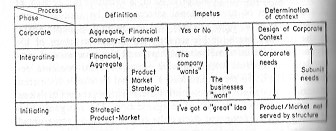
\includegraphics[width=0.85\textwidth]{Bower1970}
  \label{fig:Bower1970}
\end{centering}
\end{figure}

\begin{figure}[h]
\begin{centering}
  \caption{Types of Strategies, adopted from \cite{Mintzberg1978}}
  \includegraphics[width=\textwidth]{Mintzberg1978}
  \label{fig:Mintzberg1978}
\end{centering}
\end{figure}

\begin{figure}[h]
\begin{centering}
  \caption{Strategies form in subsystems (involving different people, skills, goals, information, and timing imperatives), adopted from \cite{Quinn1980}}
  \includegraphics[width=\textwidth]{Quinn1980a}
  \label{fig:Quinn1980a}
\end{centering}
\end{figure}

\begin{figure}[h]
\begin{centering}
  \caption{Some typical process steps in logical incrementalism (highly simplified to help visualize a few basic relationships), adopted from \cite{Quinn1980}}
  \includegraphics[width=\textwidth]{Quinn1980b}
  \label{fig:Quinn1980b}
\end{centering}
\end{figure}

\begin{figure}[h]
\begin{centering}
  \caption{Key and peripheral activities in a process model of ICV, adopted from \cite{Burgelman1983b}}
  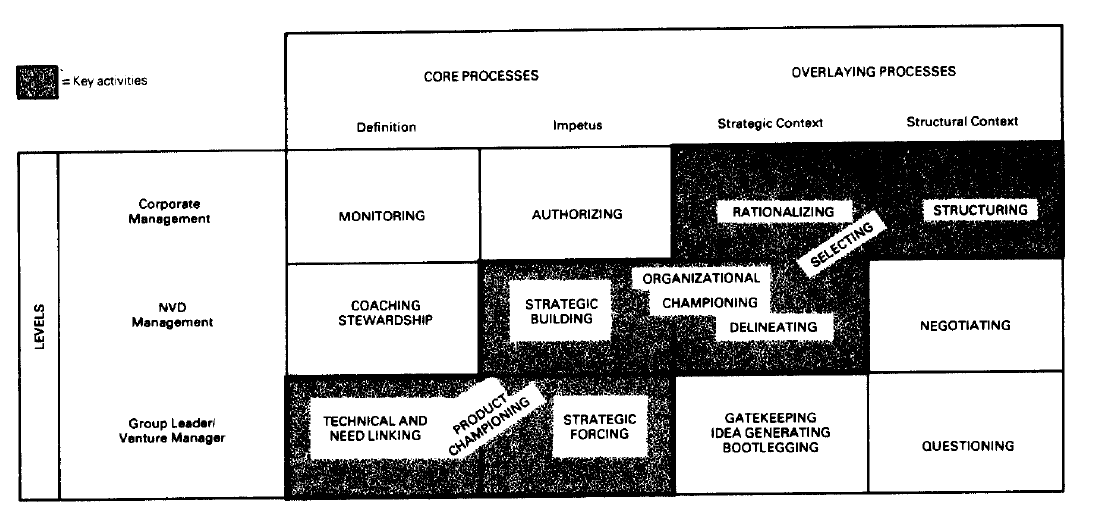
\includegraphics[width=\textwidth]{Burgelman1983b}
  \label{fig:Burgelman1983b}
\end{centering}
\end{figure}

\end{singlespace}

\end{document}
